\documentclass[journal]{IEEEtran}
%\documentclass[conference]{IEEEtran}
\hyphenation{op-tical net-works semi-conduc-tor}
\usepackage{graphicx}
\graphicspath{{./images/}}

\begin{document}
\title{Low Cost Real-time Room Occupancy Indicating System}
\author{Chirag~Shah~and~Srijal~Poojari
        \\Project~Guide:~Priya~Deshpande}


\maketitle
\begin{abstract}
The objective of this action research based project was to tackle a problem faced by corporate environments. The typical corporate office consists of several meeting rooms with employees requiring frequent access to these meeting rooms, but lack of real-time knowledge of its availability leads to inconvenient hassle. The proposed solution consists of a network of motion detection sensors (namely, the PIR sensor) spread out across all meeting rooms, updating the room occupancy status in real-time to a central base-station, a desktop computer, from which it can be relayed to the employees using a web server or a smartphone application.

Each sensor node is designed to be Low Cost, Wireless and Low Power for seamless integration and to avoid frequent battery replacement.
\end{abstract}


\section{Introduction}
\IEEEPARstart{I}{n} a typical corporate environment there exists multiple conference/meeting rooms.
The site that we studied was at Fractal Analytics, Goregaon. The office has around 400 employees: 250 employees on 7th floor, 150 employees on 3rd floor. 7th floor has 10 meeting rooms and 3rd floor has 5 meeting rooms. Anyone can book any meeting room for any time (if the room is available) using a mobile app. This is an open office - hence if anyone wants to have a discussion then they need to go to a meeting room. Hence meeting rooms are always in demand.


The problem was that anyone could book a meeting room and then not use it. Or if someone wanted to have a meeting without prebooking the meeting room the he/she would have to go from room to room to check the availability of the rooms. The would create a lot of unnecessary hassle and would lead to unoptitmal utilization of the workspace.


To solve these problem we envisioned a solution which would involve placing sensors in every meeting room to monitor the occupancy of the room. This sensor will then relay the real time occupancy information of the room to a central device which will keep track of the occupancy status of all the meeting rooms. This data can then be showed on a web/mobile interface to check the real time occupancy status of the meeting room or the data can be integrated with the the mobile app to automatically book or cancel the meetings as per the occupancy of the rooms.


\section{System Design}
\subsection{Prototype breadboards}
For testing purposes, we have designed the prototype of the circuit on breadboards which included the microcontroller, radio module and an OLED display

\begin{figure}[ht]
	\centering
	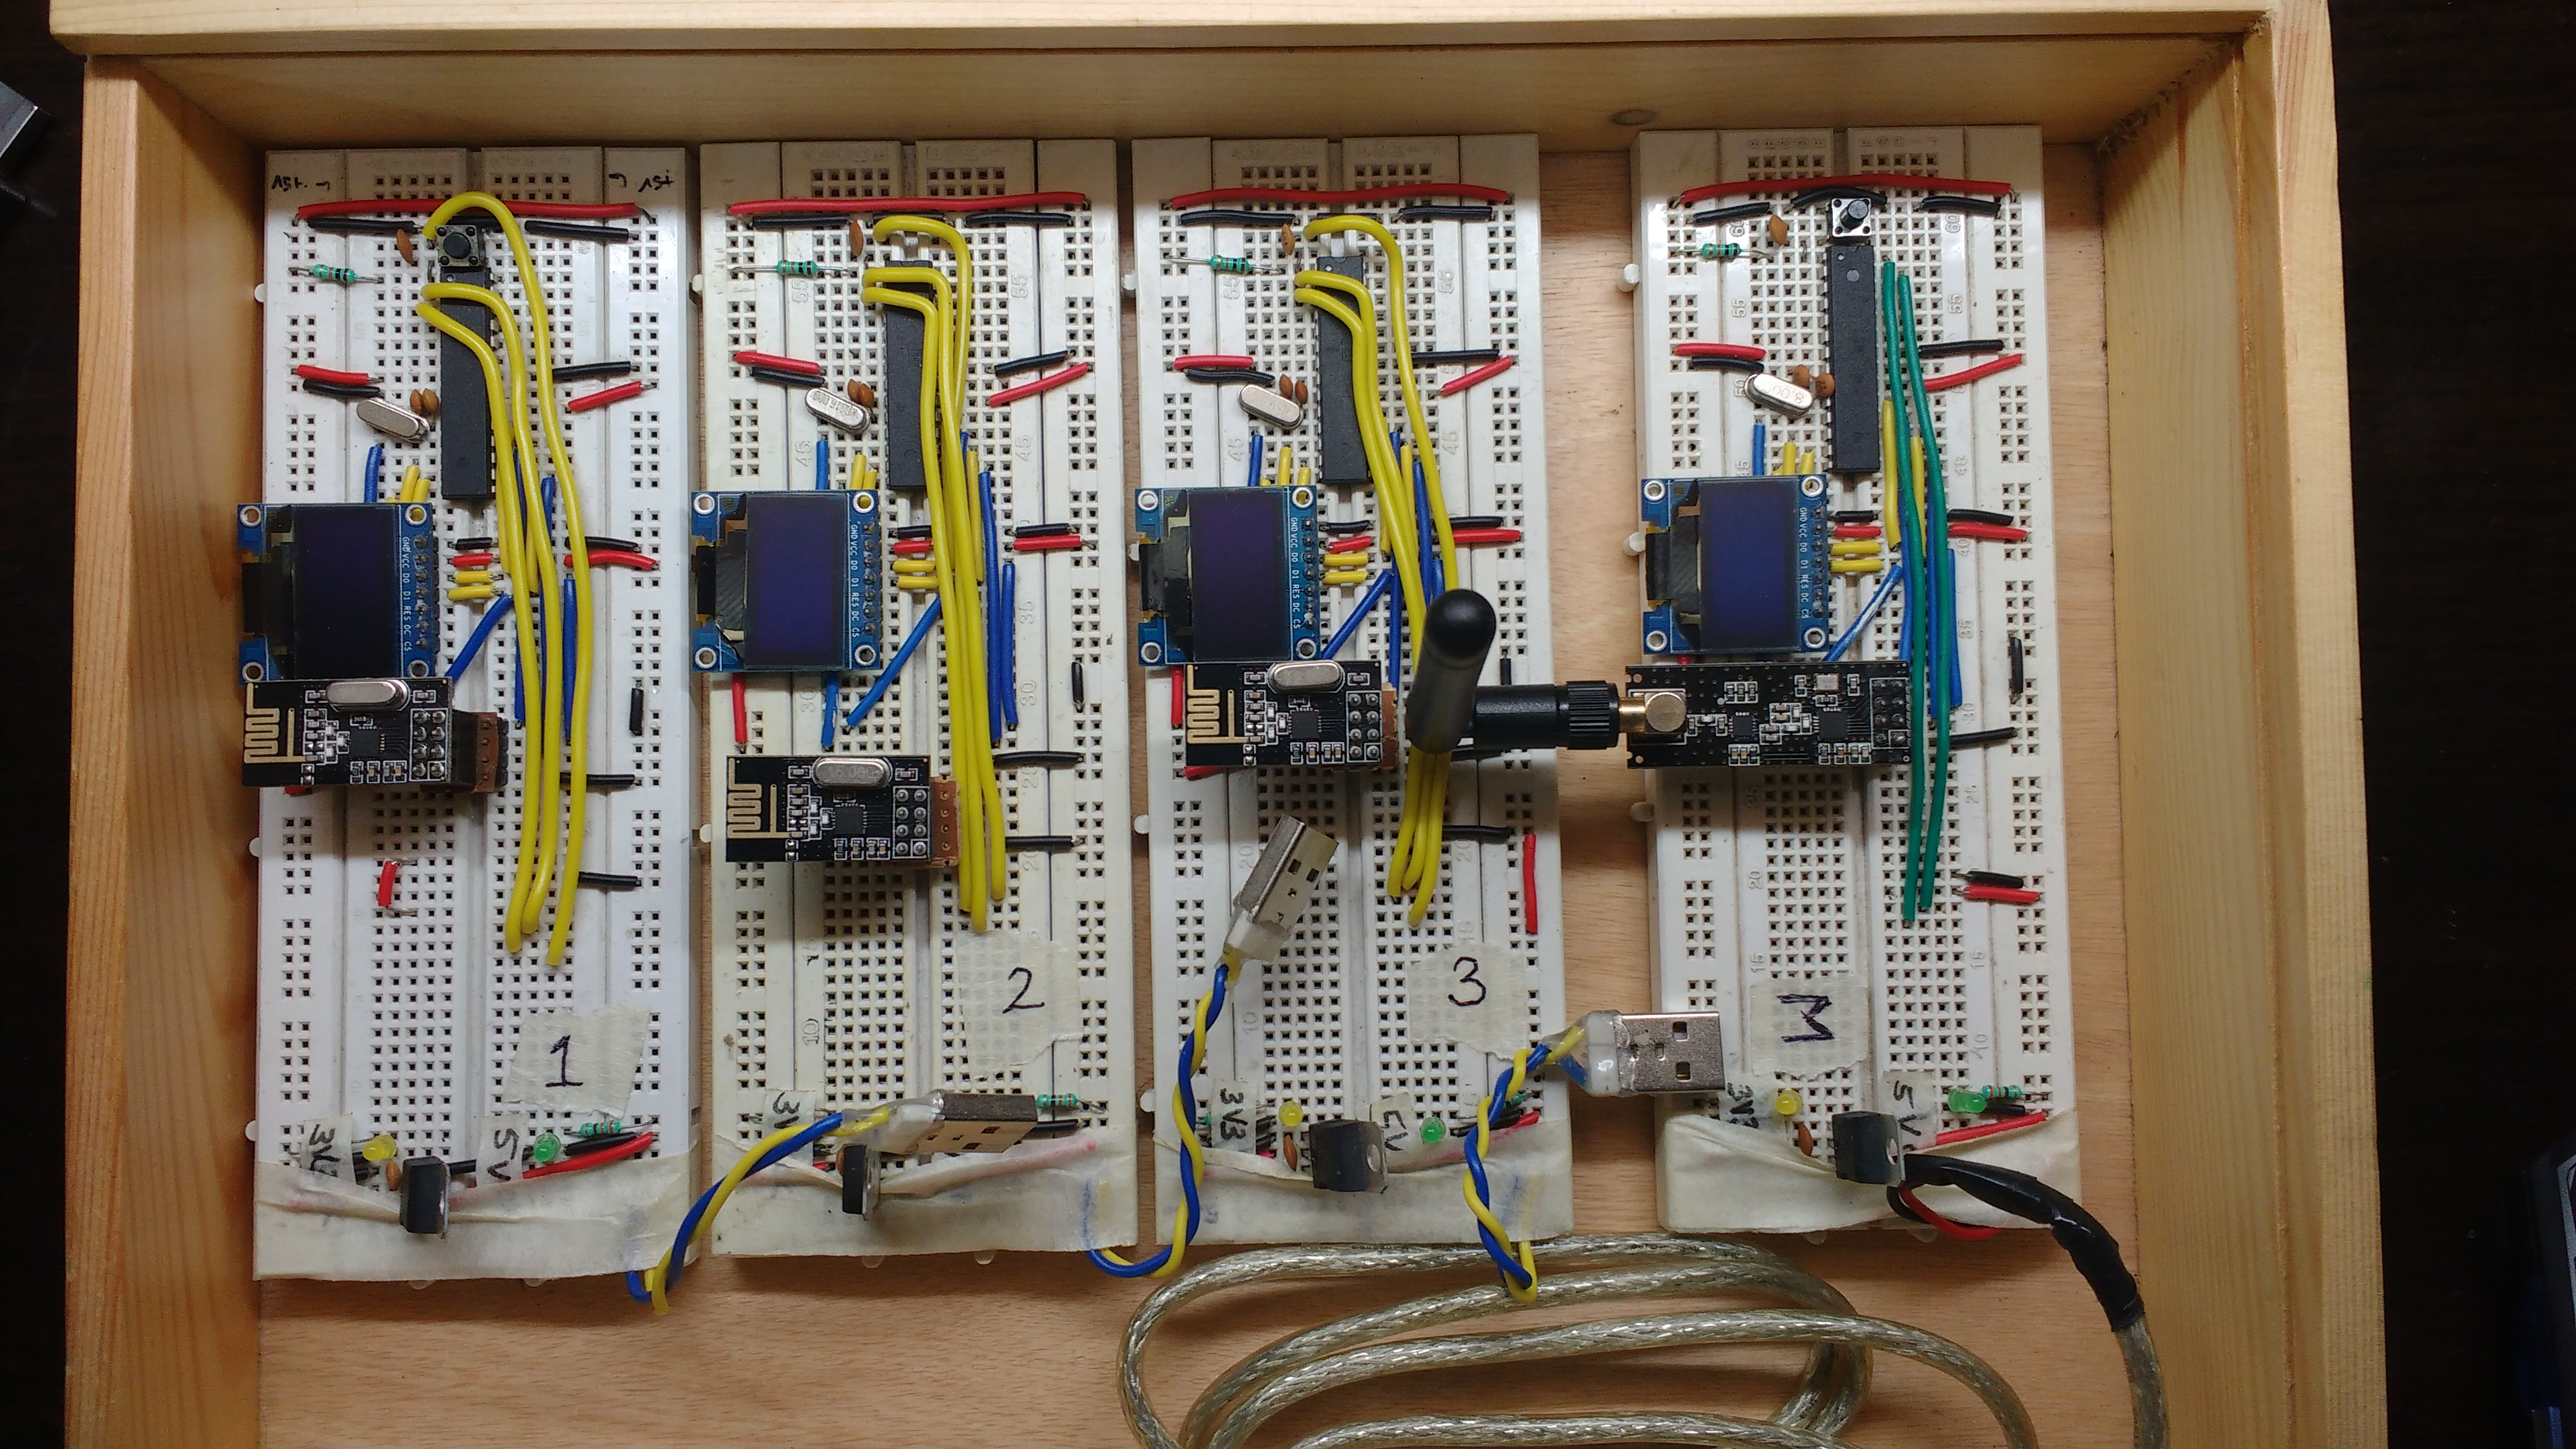
\includegraphics[scale=0.06]{all_breadboards.jpg}
	\caption{The 4 breadboard prototypes}
	\label{fig_sim}
\end{figure}

\subsection{PCBs}
Later we created PCBs using Autodesk Eagle and had it manufactured so that each node is of a small form-factor and is reliable. For this SMD components are used wherever possible. Ports for a Real Time Clock (RTC) is provided for future use in improving the low power capabilities.

\begin{figure}[ht]
	\centering
	\includegraphics[scale=0.06]{1.jpg}
	\caption{The PCB created}
	\label{fig_sim}
\end{figure}

\subsection{Enclosure}
The enclosure was designed on Autodesk Fusion 360 and 3D printed for a professional look.


\section{Results}
A frame rate of 20-25 fps is obtained when the Kinect is connected to the laptop, RTAB-Map does the mapping and RTAB-Mapviz/RViz visualizes the map. 

3-4 fps is obtained when the kinect is connected to the Raspberry Pi and mapping is done by it and the map is visualized on the laptop. The data stream from the Kinect has to be divided by two to allow the RPi to process it fast enough. RPi requires 80-100kbps bandwidth for transmitting the map over the network to the laptop.

\begin{figure}[ht]
\centering
\caption{Mapping with kinect connected to a laptop}
\label{fig_sim}
\end{figure}
 
\begin{figure}[ht]
	\centering
	\caption{Mapping with kinect connected to a laptop}
	\label{fig_sim}
\end{figure}

\newpage

\begin{figure}[ht]
	\centering
	\caption{Wireless Mapping with kinect connected to a Raspberry Pi 2}
	\label{fig_sim}
\end{figure}

\begin{figure}[ht]
	\centering
	\caption{Wireless Mapping with kinect connected to a Raspberry Pi 2}
	\label{fig_sim}
\end{figure}

\section{Conclusion}
We were able to create a wireless network of battery operated devices which which would  sense the occupancy of each room and then relay the occupancy status to a central master device. The device then relayed the real time occupancy status to a local server. A web browser (client) can then dynamically, using websockets, view the status of each node in real-time.
Future scope includes reducing the power consumption of nodes by utilizing microcontroller sleep techniques when the device is not transmitting.

\section*{Acknowledgments}

We would like to take this opportunity to thank Aashish Nehete for his immense help in creating and designing the web-based GUI for this project. We are also grateful to Prof. Kaiser Katchi for his help in 3D printing the project enclosure.
Special thanks to our institute, Sardar Patel Institute of Technology, for providing us with 3D printing services and a platform for us to showcase our project.


% Can use something like this to put references on a page
% by themselves when using endfloat and the captionsoff option.
\ifCLASSOPTIONcaptionsoff
  \newpage
\fi



% trigger a \newpage just before the given reference
% number - used to balance the columns on the last page
% adjust value as needed - may need to be readjusted if
% the document is modified later
%\IEEEtriggeratref{8}
% The "triggered" command can be changed if desired:
%\IEEEtriggercmd{\enlargethispage{-5in}}

% references section

% can use a bibliography generated by BibTeX as a .bbl file
% BibTeX documentation can be easily obtained at:
% http://mirror.ctan.org/biblio/bibtex/contrib/doc/
% The IEEEtran BibTeX style support page is at:
% http://www.michaelshell.org/tex/ieeetran/bibtex/
%\bibliographystyle{IEEEtran}
% argument is your BibTeX string definitions and bibliography database(s)
%\bibliography{IEEEabrv,../bib/paper}
%
% <OR> manually copy in the resultant .bbl file
% set second argument of \begin to the number of references
% (used to reserve space for the reference number labels box)
\begin{thebibliography}{1}

\bibitem{RTAB-Map Paper 1}
M.~Labbé and F.~Michaud, ``Memory management for real-time appearance-based loop closure detection,"
in \emph{Proceedings of the IEEE/RSJ International Conference on Intelligent Robots and Systems}, 2011, pp. 1271–1276.

\bibitem{Programming Robots with ROS}
Morgan Quigley, Brian Gerkey, William D. Smart, \emph{Programming Robots with ROS}. 2016, p. 3.

\bibitem{What is ROS- Quora}
Po Jen Lai, ``What is ROS? [Online]. Available: 
https://www.quora.com/What-is-ROS
[Accessed: 31- Oct- 2017].

\bibitem{What is ROS- Quora}
Zeeshan Khan S, ``What is ROS?" [Online]. Available: 
https://www.quora.com/What-is-ROS
[Accessed: 31- Oct- 2017].

\bibitem{ROS Nodes}
ROS.org, ``Nodes." ROS wiki [Online]. Available: http://wiki.ros.org/Nodes

\bibitem{RTB-Map}
Mathieu Labbé, ``Overview on RTAB-Map." [Online]. Available: 
http://introlab.github.io/rtabmap/
[Accessed: 31- Oct- 2017].

\end{thebibliography}

\end{document}


